\documentclass[a4paper,12pt]{article}

\usepackage{amsmath,amssymb,multicol,tikz,enumitem}
\usepackage[margin=2cm]{geometry}
%\usetikzlibrary{calc}
\usepackage{amsmath}
\usepackage{amsthm}
\usepackage{thmtools}
\usepackage{hyperref}
\usepackage{enumerate}
\usepackage{xcolor}
\usepackage{fancyvrb}

\pagestyle{empty}

\newcommand\Q{\mathbf{Q}}
\newcommand\R{\mathbf{R}}
\newcommand\Z{\mathbf{Z}}

\usepackage{array}
\newcolumntype{P}[1]{>{\centering\arraybackslash}p{#1}}

\newcommand\indd{${}$\hspace{20pt}}

\declaretheoremstyle[headfont=\normalfont\bfseries,notefont=\mdseries\bfseries,bodyfont = \normalfont,headpunct={:}]{normalhead}
\declaretheorem[name={Uzdevums}, style=normalhead,numberwithin=section]{problem}

\setcounter{section}{112}

\setlength\parindent{0pt}

\begin{document}

\clearpage
\begin{center}
\parbox{3.5cm}{\flushleft\bf Visādas olimpiādes \newline ATV} \hfill {\bf\LARGE Uzdevumu lapa \#12} \hfill \parbox{3.5cm}{\flushright\bf 2021-03-24} %\\[2pt]
\end{center}

%\hrule\vspace{2pt}\hrule
\hrule


%AMO2009.12.5. 
\vspace{10pt}
\begin{problem}
Uz galda atrodas $n$ konfektes, $n$ – naturāls skaitlis. Divi spēlētāji pamīšus ēd pa $x^2$ konfektēm, 
kur $x$ – naturāls skaitlis ($x$ var mainīties no gājiena uz gājienu). 
Tas, kam nav ko ēst, zaudē. Pierādīt: ir bezgalīgi daudz tādu $n$, 
ka, pareizi spēlējot, otrais spēlētājs var uzvarēt.
\end{problem}

%AMO.2010.11.5. 
\vspace{10pt}
\begin{problem}
Naturālu skaitli $n$ sauksim par sakarīgu, ja eksistē slēgta lauzta līnija ar $n$ posmiem, 
kura katru savu posmu krusto tieši $2$ reizes. Tā piemēram, $5$ ir sakarīgs 
skaitlis, skat.\ Attēlu~\ref{fig:star}. Noskaidro, kādiem naturāliem $k$ skaitlis $2^k$ ir sakarīgs!
\begin{figure}[!htb]
\center{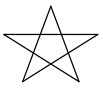
\includegraphics[width=1in]{atv-12/star.png}}
\caption{\label{fig:star} Lauzta līnija ar $n=5$ posmiem, katru posmu krusto tieši divreiz.}
\end{figure}
\end{problem}

%AMO.2011.11.3.
\vspace{10pt}
\begin{problem}
Cik veidos taisnstūri ar izmēriem $3 \times 12$ rūtiņas var sadalīt taisnstūros ar izmēriem $1 \times 3$ rūtiņas? 
(Dalījuma līnijām jāiet pa rūtiņu malām, taisnstūri var būt novietoti gan horizontāli, gan vertikāli.)
\end{problem}


%AMO.2012.12.5.
\vspace{10pt}
\begin{problem}
Klasē ir $17$ skolēni. Katru dienu daži no viņiem (vismaz viens) tiek izsaukti pie tāfeles. 
Kāds ir mazākais dienu skaits, pēc kurām ir iespējams, ka katriem diviem klases skolniekiem 
ir bijusi diena, kad viens no viņiem ir izsaukts pie tāfeles, bet otrs nē?
\end{problem}


%AMO.2013.12.4. 
\vspace{10pt}
\begin{problem}
Kādas valodas alfabētā ir $i$ patskaņi ($i \geq 2$) un $j$ līdzskaņi ($j \geq 2$). 
Šajā valodā par vārdu sauc jebkuru galīgu burtu (patskaņu un līdzskaņu) virkni, 
kas satur vismaz vienu burtu un kurā nekādi divi patskaņi neparādās pēc kārtas 
un pēc kārtas uzrakstīti līdzskaņi ir ne vairāk kā divi (piemēram, ja ``A'' ir patskanis, 
bet ``B'' – līdzskanis, tad, piemēram, ``ABBA'' ir vārds, turpretī ``BAAB'' un ``ABBBA'' nav vārdi). 
Ar $S(n)$ apzīmēsim visu to vārdu skaitu, kuri sastāv no $n$ burtiem, $n \geq 1$. 
Pierādīt, ka visiem naturāliem skaitļiem $n$ ir spēkā vienādība
\[ S(n+3) = i \cdot j \cdot S(n+1) + i \cdot j^2 \cdot S(n). \]
\end{problem}




\end{document}

